\chapter{Theoretical Background}
This chapter covers the theoretical background
needed to understand sleep staging.
We begin by describing the different stages
of sleep and the electroencephalogram (EEG) patterns
that are used to define them. We then explain the official
AASM guidelines, which provide the standardized rules
for classifying these sleep stages. These are heavily
used by sleep technicians in clinical practice and
help us understand how sleep staging is performed manually.

\section{Understanding Sleep Stages}
Sleep is an important physiological process that is essential for our overall health.
Since the quality of our sleep directly affects how we function during our waking hours,
it has been the subject of extensive scientific study. Far from being a uniform state,
sleep is organized into a predictable pattern of distinct stages, collectively known as
sleep architecture. The analysis of this architecture is performed through a process
called sleep staging, where a continuous overnight recording is segmented into 30-second epochs,
each of which is classified into a specific stage.

The American Academy of Sleep Medicine (AASM) recognizes five distinct stages of sleep \cite{AASM}:
\begin{itemize}
    \item Wake (W)
    \item Rapid Eye Movement (REM) sleep
    \item Non-Rapid Eye Movement (NREM) sleep, which is further divided into three stages:
    \begin{itemize}
        \item N1 (Stage 1)
        \item N2 (Stage 2)
        \item N3 (Stage 3)
    \end{itemize}
\end{itemize}

In a healthy adult, sleep typically progresses through the stages in a repeating cycle: from N1 to N2 and N3,
then back to N2, and finally into REM. Each of these cycles lasts about 90 minutes \cite{Patel2025Physiology}.

To understand the properties of each stage, we must first define EEG frequency bands commonly used \cite{AASM}. These are:
\begin{itemize}
    \item Delta waves: Waves in range of 0–3.99 Hz. 
    \item Theta waves: Waves in range of 4–7.99 Hz.
    \item Alpha waves: Waves in range of 8–13 Hz.
    \item Beta waves: Waves greater than 13 Hz.
\end{itemize}

Wakeful stage (W) shows different patterns depending on whether subjects eyes are open or closed.
During eye-open wakefulness, beta waves predominate. Alpha waves become predominant as individuals
become drowsy and close their eyes \cite{Patel2025Physiology}.

N1 stage is a short light stage of sleep, lasting around 1–5 minutes at a time. Only around 5\% of total sleep time is spent in this stage.
During this stage more than half of the alpha waves are replaced with low-amplitude mixed-frequency (LAMF) activity (predominantly 4–7 Hz activity).

N2 stage, also called "deeper sleep" is the most common sleep stage, accounting for approximately 45\% of total sleep time in adults.
During this stage heart rate and body temperature drop. It is additionally characterized by the presence of "sleep spindles" - 
brief, powerful bursts of neuronal firings and "K-complexes" - delta waves that last approximately one second.
N2 sleep lasts around 25 minutes in the first sleep cycle and lengthens with each successive cycle \cite{Patel2025Physiology}.

N3 sleep consists of 25\% of total sleep time. This is considered the deepest stage of sleep, 
characterized with the presence of delta waves. This is the stage when the body repairs and 
regrows tissues, builds bone and muscle, and strengthens the immune system.
With age, people spend less time in N3 sleep and more time in stage N2 \cite{Patel2025Physiology}.

Finally, REM (Rapid Eye Movement) sleep consists of 25\% of total sleep time. Famously,
this is the stage when dreaming occurs. Brain activity increases, as 
beta waves predominate during this stage, resembling that of wakefulness.
First cycle typically lasts around 10 minutes, with each successive REM stage lengthening,
with the final one lasting up to an hour \cite{Patel2025Physiology}.
As name suggests, this stage is characterized by rapid movement of the eyes under closed eyelids.

\section{Sleep Staging Guidelines}
The clinical practice of sleep staging is governed by the guidelines set forth in The AASM Manual for the Scoring of Sleep and Associated Events \cite{AASM}.
The guideline proposes a set of rules for sleep staging for adults, children and infants. These also specify rules 
for EOG (electrooculogram) and EMG (electromyogram) signal usage in sleep staging, which are not covered in this thesis.

\begin{figure}[h!]
    \centering
    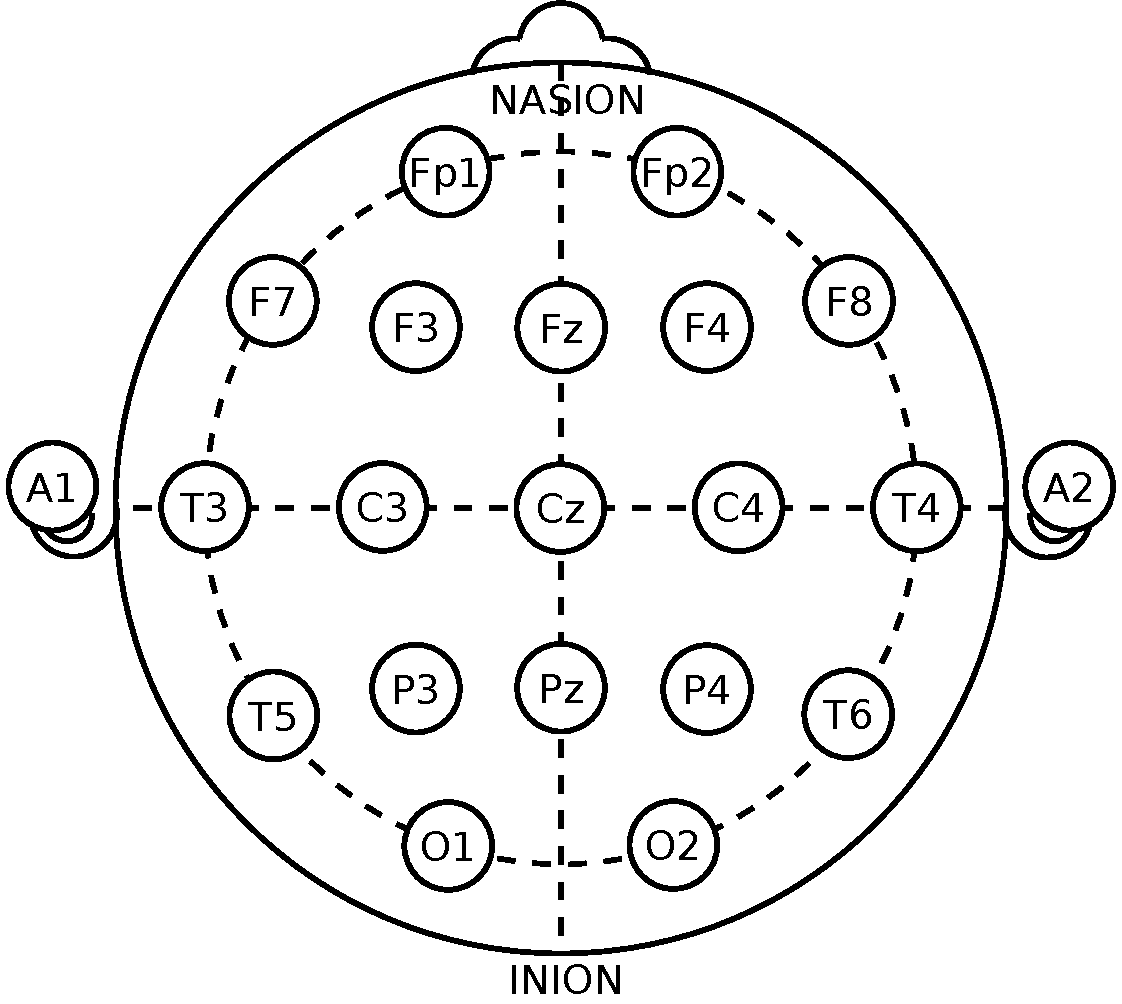
\includegraphics[width=0.8\textwidth]{EEG_Cap.pdf}
    \caption{The standard placement of 21 electrodes according to the International 10-20 system for an electroencephalogram (EEG). The M1 node is equal to A1. Image retrieved from Wikimedia Commons, is in the public domain.}
    \label{fig:eeg_electrodes}
\end{figure}

The AASM \cite{AASM} recommends the following EEG derivations for sleep staging, known as a \textbf{referential montage}:
\begin{itemize}
    \item F4-M1
    \item C4-M1
    \item O2-M1
\end{itemize}
A derivation is a pair of electrodes, for which we measure the difference in voltage between them.
In the above list, the first electrode is placed on the right side of the head, while the second electrode is placed on the left mastoid process.

AASM \cite{AASM} requires that at minimum three derivations are used for sleep staging. Additionally, it prescribes backups, 
if any of nodes fail. For example M1 can be replaced with M2.

It is standard to split EEG data into 30-second epochs. Each epoch is then classified into one of the five sleep stages (W, N1, N2, N3, REM)
If an epoch contains characteristics of multiple stages, the stage that occupies the majority of the epoch is assigned.

Same electrode derivations can be used for children (older than 2 months post-term). However, 
sleep stages can differ. If non-REM sleep is not sufficiently developed (if recording does not contain sleep spindles or
K-complexes), AASM \cite{AASM} recommends using a simplified stage N.
Sleep spindles can appear as early as 6 weeks post-term and are present in all infants by age of 3 months.
However, K-complexes start to appear between 3 and 6 months of age \cite{AASM}. That means, that by age of 
6 months, stage N can be fully divided into N1, N2 and N3 sleep for most children.

For infants (younger than 2 months post-term), AASM \cite{AASM} prescribes a different set of sleep stages:
\begin{itemize}
    \item Wakefulness (W)
    \item Non-REM sleep (N)
    \item REM sleep (R)
    \item Transitional sleep (T)
\end{itemize}
Historically, these stages were often referred to as quiet sleep (N), active sleep (R), and indeterminate sleep (T) \cite{AASM}.

Properties of these stages differ from those in older children and adults. For example, non-REM sleep
can be characterized by Trace alternant pattern - at least 3 alternating runs of high voltage delta waves
lasting 5 to 6 seconds, followed by low voltage theta waves lasting for 4 to 12 seconds.
Non-REM sleep mostly consists of high voltage slow wave activity (delta waves predominating). However,
high voltage slow wave activity can also be present in REM sleep \cite{AASM}. If NREM stage is sufficiently
developed, this stage can already be classified into N1, N2 and N3 sleep. In that case, staging rules for children apply.

On the other hand, REM sleep can be characterized by low voltage mixed frequency activity (delta and theta waves predominating).

To account for the ambiguity of infant sleep patterns, the AASM defines \textbf{Stage T}. This stage is scored when
an epoch contains 3 Non-REM characteristics and 2 REM characteristics, or 2 Non-REM characteristics and 3 REM characteristics \cite{AASM}.
Transitional stage aids the staging process, as sleep stages in infants are not yet fully developed.